\problemname{Beautiful Subsets}

We are given a tree with $n$ vertices, numbered from $1$ to $n$. Each vertex is
colored with one of $b$ possible colors (the colors are represented by the
integers from $1$ to $b$).

We say that a subset of vertices $A \subseteq \{1, 2, \ldots, n\}$ is
\emph{beautiful} if:
\begin{itemize}
  \item all vertices in $A$ have the same color, and
  \item there exists a simple path in the tree (that visits no vertex more than
        once) that visits all vertices in $A$ (it may also visit some vertices
        that are not in $A$).
\end{itemize}

Write a program that, for each color, finds the size of the largest beautiful
subset consisting of vertices of that color.

\begin{figure}[h]
  \centering
  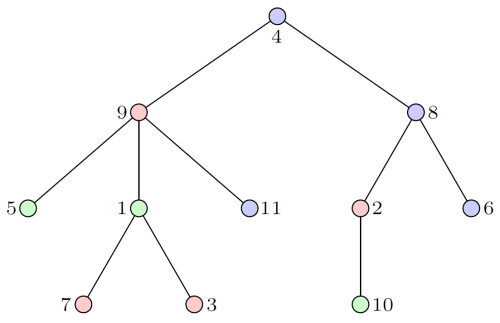
\includegraphics[width=0.6\textwidth]{subsets-tree}
  \caption*{A tree with $n = 11$ vertices and $b = 3$ colors that corresponds to
  the first example input.}
\end{figure}

\section*{Input}
The first line contains two integers, $n$ (the number of vertices) and $b$ (the
number of colors), separated by a space. The remainder of the input depends on
the value of $n$:
\begin{itemize}
  \item If $n \leq 200\,000$ (which holds for the first three subtasks), the
        first line (the one containing $n$ and $b$) is followed by $n$ more
        lines. The $i$-th of these lines contains two integers, $p_i$ and $c_i$,
        indicating that vertex $i$ has color $c_i$ and parent $p_i$. If $i$ is
        the root of the tree and therefore has no parent, then $p_i = 0$. (For
        example, in the figure above, vertex $9$ is the parent of vertices $1$,
        $5$, and $11$, while vertex $4$ is the root of the tree.)
  \item If $n > 200\,000$ (which occurs only in the fourth subtask), the first
        line is followed by a single additional line containing seven numbers
        separated by spaces: $A$, $B$, $M$, $K$, $A'$, $B'$, and $M'$. These are
        integers between $1$ and $10^9$. They define two sequences:
        \[ r_0 = 0, \quad r_{i+1} = (A \cdot r_i + B) \bmod M \]
        \[ r'_0 = 0, \quad r'_{i+1} = (A' \cdot r'_i + B') \bmod M' \]
        Such an input represents a tree with the following values. Vertex $1$ is
        the root (so $p_1 = 0$). For each $i = 2, \ldots, n$, vertex $i$ has
        parent $p_i = i - 1 - \left( r_i \bmod \min(K, i-1) \right)$. For each
        $i = 1, \ldots, n$, vertex $i$ has color $c_i = 1 + (r'_i \bmod b)$.
        (The purpose of these formulas is to allow us to provide a large,
        approximately random tree without requiring you to read an enormous
        amount of input data.)
\end{itemize}

The following limits hold:
\begin{itemize}
  \item $1 \leq b \leq n \leq 5\,000\,000$
  \item For every $i$, we have $1 \leq p_i \leq n$ (except for the root, where
        $p_i = 0$) and $1 \leq c_i \leq b$.
  \item The parent data $p_i$ is such that the edges between vertices and their
        parents indeed form a tree.
\end{itemize}

\section*{Output}
Let $\ell_i$ denote the size of the largest beautiful subset containing vertices
of color $i$. The required output of your program depends on the value of $n$:
\begin{itemize}
  \item If $n \leq 200\,000$, print $b$ lines. On the $i$-th line (for each
        $i = 1, \ldots, b$), print the value $\ell_i$ (i.e. the size of the
        largest such beautiful subset containing vertices of color $i$).
  \item If $n > 200\,000$, print a single line containing the sum
        $\ell_1 + \ell_2 + \cdots + \ell_b$. (The purpose of this requirement is
        to avoid producing a huge amount of output for large test cases.)
\end{itemize}

\section*{Scoring}
Your solution will be tested on a set of test groups.
To earn points for a group, you must pass all test cases in that group.

\noindent
\begin{tabular}{| l | l | p{12cm} |}
  \hline
  \textbf{Group} & \textbf{Points} & \textbf{Constraints} \\ \hline
  $1$ & $25$ & $n \leq 20$ \\ \hline
  $2$ & $25$ & $n \leq 1\,000$ \\ \hline
  $3$ & $30$ & $n \leq 200\,000$ \\ \hline
  $4$ & $20$ & No additional constraints. \\ \hline
\end{tabular}

\section*{Explanation of Samples}
The first sample corresponds to the figure above. For color $1$, for instance,
there exists a beautiful subset $\{2, 7, 9\}$, which can be visited by the path
$2 \rightarrow 8 \rightarrow 4 \rightarrow 9 \rightarrow 1 \rightarrow 7$.
